\documentclass[output=paper]{langsci/langscibook}
\usepackage{fontspec}

\author[Yang Xu and Zheng-sheng Zhang]{Yang Xu {\cjkfont 徐炀}\orcid{}\affiliation{San Diego State University}  and
Zheng-sheng Zhang {\cjkfont 张正生}\orcid{}\affiliation{San Diego State University}}


\title{Historical changes in semantic weights of sub-word units}

\abstract{In this chapter, we present a computational study on how the weight of sub-word units in determining word meanings evolves chronologically in different languages. Sub-word units, e.g., morphemes, syllables etc., play variable roles in determining word meanings. Some morphemes in English have standalone lexical meanings (e.g., the root) while others function more as morpho-syntactic markers (e.g., the bound morphemes such as -\textit{ness} etc.) The semantic weight of sub-word units changes over time; for instance, some ancient characters in Chinese or ancient prefixes in English no longer carry clear semantic meanings. The goal of this chapter is to characterize such a change with computational methods. The semantic weight of sub-word units can be captured by word embedding models (and their variants). 

We present results from two substudies. In Study 1, we propose a novel neural network-based word embedding model to model the semantic weights from sub-word units. We draw a comparison between Chinese and Indo-European languages in how the semantic weights of sub-words change over time, and show that the weights of characters in Chinese ({\cjkfont 字} \textit{zi}, the basic sub-word unit in Chinese) are higher in ancient Chinese and lower in modern Chinese, while the opposite trend is observed in Indo-European languages. This is in accordance with theories about monosyllabic-to-bisyllabic shift in Chinese, and the synthetic-to-analytic shift conjecture in Indo-European languages. 
In Study 2, we apply a different embedding model on another corpus to confirm the finding in Study 1. Although the chronological pattern of semantic weight found is inconsistent with that in Study 1, the results are still meaningful in having discovered the presence of historical changes of sub-word level semantic weights across different corpora and languages. 

Our chapter calls for more systematic studies of the applicability of computational embedding methods in modeling the sub-word semantics. Although discrepancies are found in current models and corpora, our empirical findings suggest that word level semantic composition is a dynamic process which reflects historical changes.}
 
\begin{document}
\SetupAffiliations{mark style=none}
\maketitle


%Transcriptions of Chinese characters:

%字 => zi
%教育 => jiao yu, 教 => jiao, 育 => yu
%爱人 => ai ren, 爱 => ai, 人 => ren
%中书 => zhong shu, 中 => zhong, 书 => shu
%一 => yi, 三 => san, 万 => wan
%一定 => yi ding, 定 => ding
%不能 => bu neng, 不 => bu, 能 => neng
%世事 => shi shi, 世 => shi, 事 => shi
%士大夫 => shi da fu, 士 => shi, 大 => da, 夫 => fu
%皇太后 => huang tai hou, 皇 => huang, 太 => tai, 后 => hou
%都督府 => du du fu, 都 => du, 督 => du,  府 => fu



\section{Introduction}

The roles that sub-word units play in determining word semantics differ across languages. In typical alphabetic languages, such as English, the smallest grammatical sub-word unit is \emph{morpheme} \citep{katamba2015english}. A morpheme is either free or bound: the former stands by itself as a word (e.g., the \emph{root} of English words), while the latter functions only as part of a word (e.g., \emph{affixes} such as \emph{-ness}, \mbox{\emph{un-},} etc.). 
In East-Asian languages, however, the distinction between morphemes and words is not as clear. Particularly in Chinese, the basic sub-word unit that acts as a morpheme is the character ({\cjkfont 字} \textit{zi}), but whether a single morpheme or a combination of morphemes constitute a word is open to debate \citep{hsieh2016chinese}. 

In this chapter, we present two studies that use sub-word incorporated word embeddings to explore the temporal patterns of the semantic weight of sub-word units. 
In \Cref{sec:study1}, we present our first study, in which a novel \textsc{dynamic sub-word-incorporated embedding} (DSE) model is proposed, which quantifies the semantic weights of sub-word units automatically via joint training tasks. The advantage of this method is that the weights for different words are modeled separately, which provides more fine-grained information. 
In \Cref{sec:study2}, we present the second study, in which we examined the existing model \textsc{character-enhanced word embedding} (CWE) to obtain sub-word embeddings, and then computed the semantic weights by comparing the norms of sub-word vectors with word vectors. This method leads to faster training and more interpretable results. The purpose of the second study is to confirm whether consistent findings can be reached with a different model and corpus.
With these two studies, our goal is to reach reliable conclusions with computational approaches about how the semantic weights of sub-word units change historically. 


\section{Related work}
\subsection{Learning vector representations of words}
Among the massive amount of approaches to learning dense word vectors, one of the most popular methods is the word2vec model, which implements two efficient ways of learning word vectors, skipgram and CBOW (continuous bag of words) \citep{mikolov2013-distributed,mikolov2013efficient}. Both models learn word embeddings by training a network to predict words that co-occur within a window. 
CBOW aims at predicting  the target word given context words in a fixed window, while skipgram predicts the context word given the target word at the center, by maximizing the probability of target/context word, which is approximated with hierarchical softmax or negative sampling \citep{mikolov2013-distributed,mikolov2013efficient}.


\subsection{Word embeddings with sub-word information}\label{sec:improve_sub-word}
For most languages in the world, the internal structure of words contains information about the semantics of the word. 
Incorporating parameters associated with those internal structures in the training process can improve word embeddings so that they are more expressive of the meanings of words. 
There are two types of improvement, semantic compositionality and reducing sparsity. Some languages have strong compositionality at the word level. In Chinese for example, the meaning of a word can be inferred by assembling the meanings of all characters. For instance, the word {\cjkfont 教育} \textit{jiao yu} `education', can be inferred from the meanings of its first character {\cjkfont 教} \textit{jiao} `teach' and second character {\cjkfont 育} \textit{yu} `raise'. 
Based on this, \citet{chen2015joint} propose a character-enhanced word embedding model (CWE) 

The second type of improvement uses the fact that in some morphologically rich languages, one word can have multiple forms that occur rarely, making it difficult to learn good representations for them. 
For example, Finnish has 15 cases for nouns,\footnote{See \url{http://jkorpela.fi/finnish-cases.html}.} while French or Spanish have more than 40 different inflected forms for most verbs. 
A way to deal with this sparsity issue is to use sub-word information. \citet{bojanowski2017enriching} propose to learn representations for character \emph{n}-grams and represent words as the sum of their \emph{n}-gram vectors.\footnote{Another approach is to tokenize words into sub-words while optimizing a language model acquired over these \emph{word pieces} \citep{schuster2012japanese,sennrich2015neural}.}
Their model, \emph{fastText}, alters the training objective of skipgram by replacing the target word vector with the sum of its \emph{n}-gram vectors. 


\subsection{Word embeddings and language change}
Word vectors have been used to study the long-term change of languages from multiple angles. 
The most straightforward method is to group text data into time bins and then train embeddings separately on these bins \citep{kim-etal-2014-temporal,kulkarni2015statistically,hamilton-etal-2016-diachronic}. Conclusions about language change are reached by observing how the vectors of the same words change over time. The problem with this approach is that the learned word vectors are subject to random noise due to corpus size. 
\citet{bamler17} address this with a probabilistic variation of word2vec model, in which words are represented by latent trajectories in the vector space, and the semantic shift of words is described by a latent diffusion process through time. 
Most of the existing approaches describe language change by the trajectories of some representations in a high dimensional space. Even though this provides rich information about every single point in the space (word, character etc.), it is difficult to interpret and summarize these models and discover the general patterns of language change.
Other studies using word embeddings or related methods have been used in very similar context \citep{tahmasebi2018survey,kutuzov-etal-2018-diachronic}.
This chapter explores the historical changes of sub-word level semantics, which has not been studied extensively in existing computational studies.


\section{Study 1: Relationship between semantic weight and word age}\label{sec:study1}

\subsection{Dynamic sub-word-incorporated embedding model (DSE)}\label{sec:DSE}
We propose the dynamic sub-word-incorporated embedding (DSE) model, which captures the semantic weights carried by the sub-word units in words, on top of the architecture of CWE and fastText models. 
The ``dynamic'' part is reflected in the design considering that words rely on their internal structures to different degrees in composing a meaning: we associate each word in the vocabulary with a scalar parameter $h^w$, within the range $[0,1]$, which is the weight of the word itself in predicting the co-occurring words within a context window. Correspondingly, $1-h^w$ is the weight of its sub-word units. 
Here the sub-word units refer to characters in a Chinese word, and a subset of $n$-grams of a word for English and four other languages used in this study. 
We did not use word roots and affixes as the sub-word units as in \citet{xu2018incorporating}, because of the lack of dictionary data in some languages, and the relative simplicity of $n$-gram-based models. 


\begin{figure*}[h]
\centering
\begin{subfigure}{0.66\linewidth}
	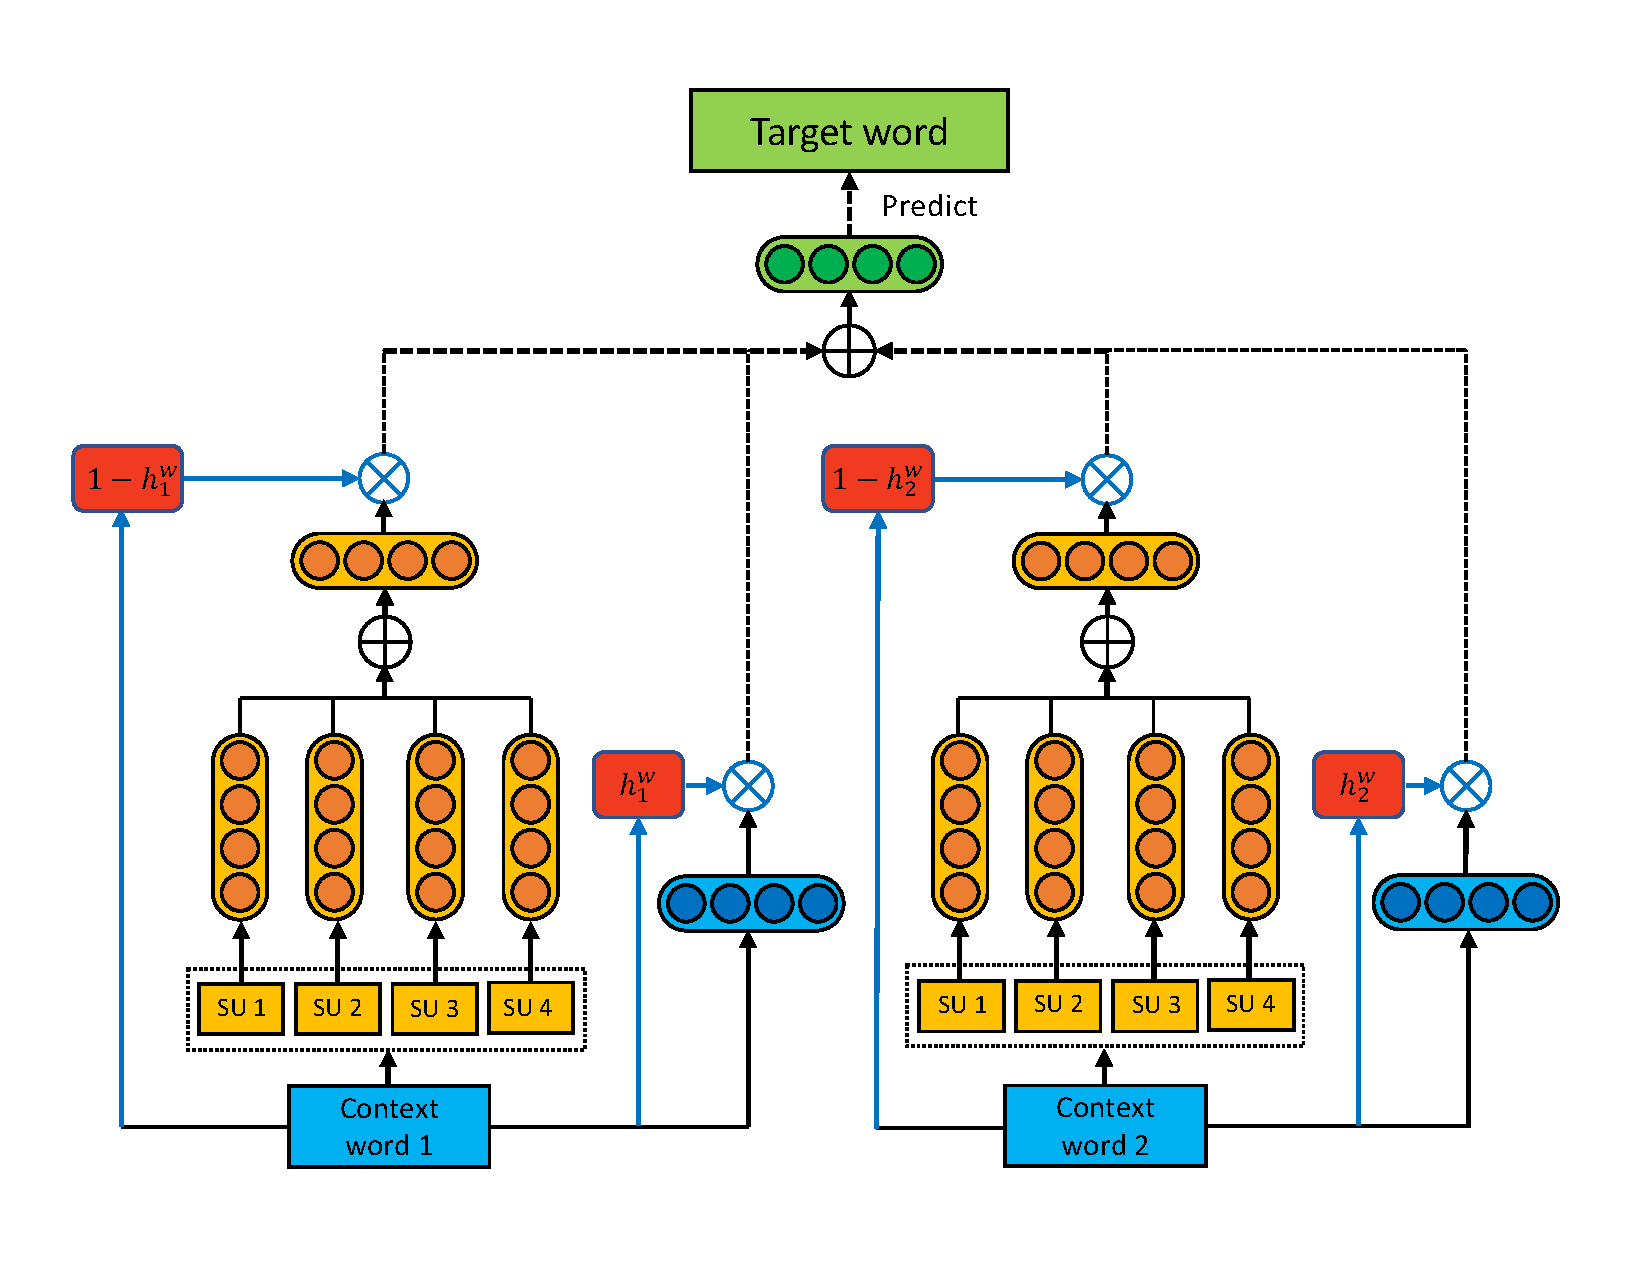
\includegraphics[width=\textwidth]{figures/XU_DSE-CBOW_subword.pdf}
	\caption{DSE-CBOW}
\end{subfigure}
\begin{subfigure}{0.33\linewidth}
	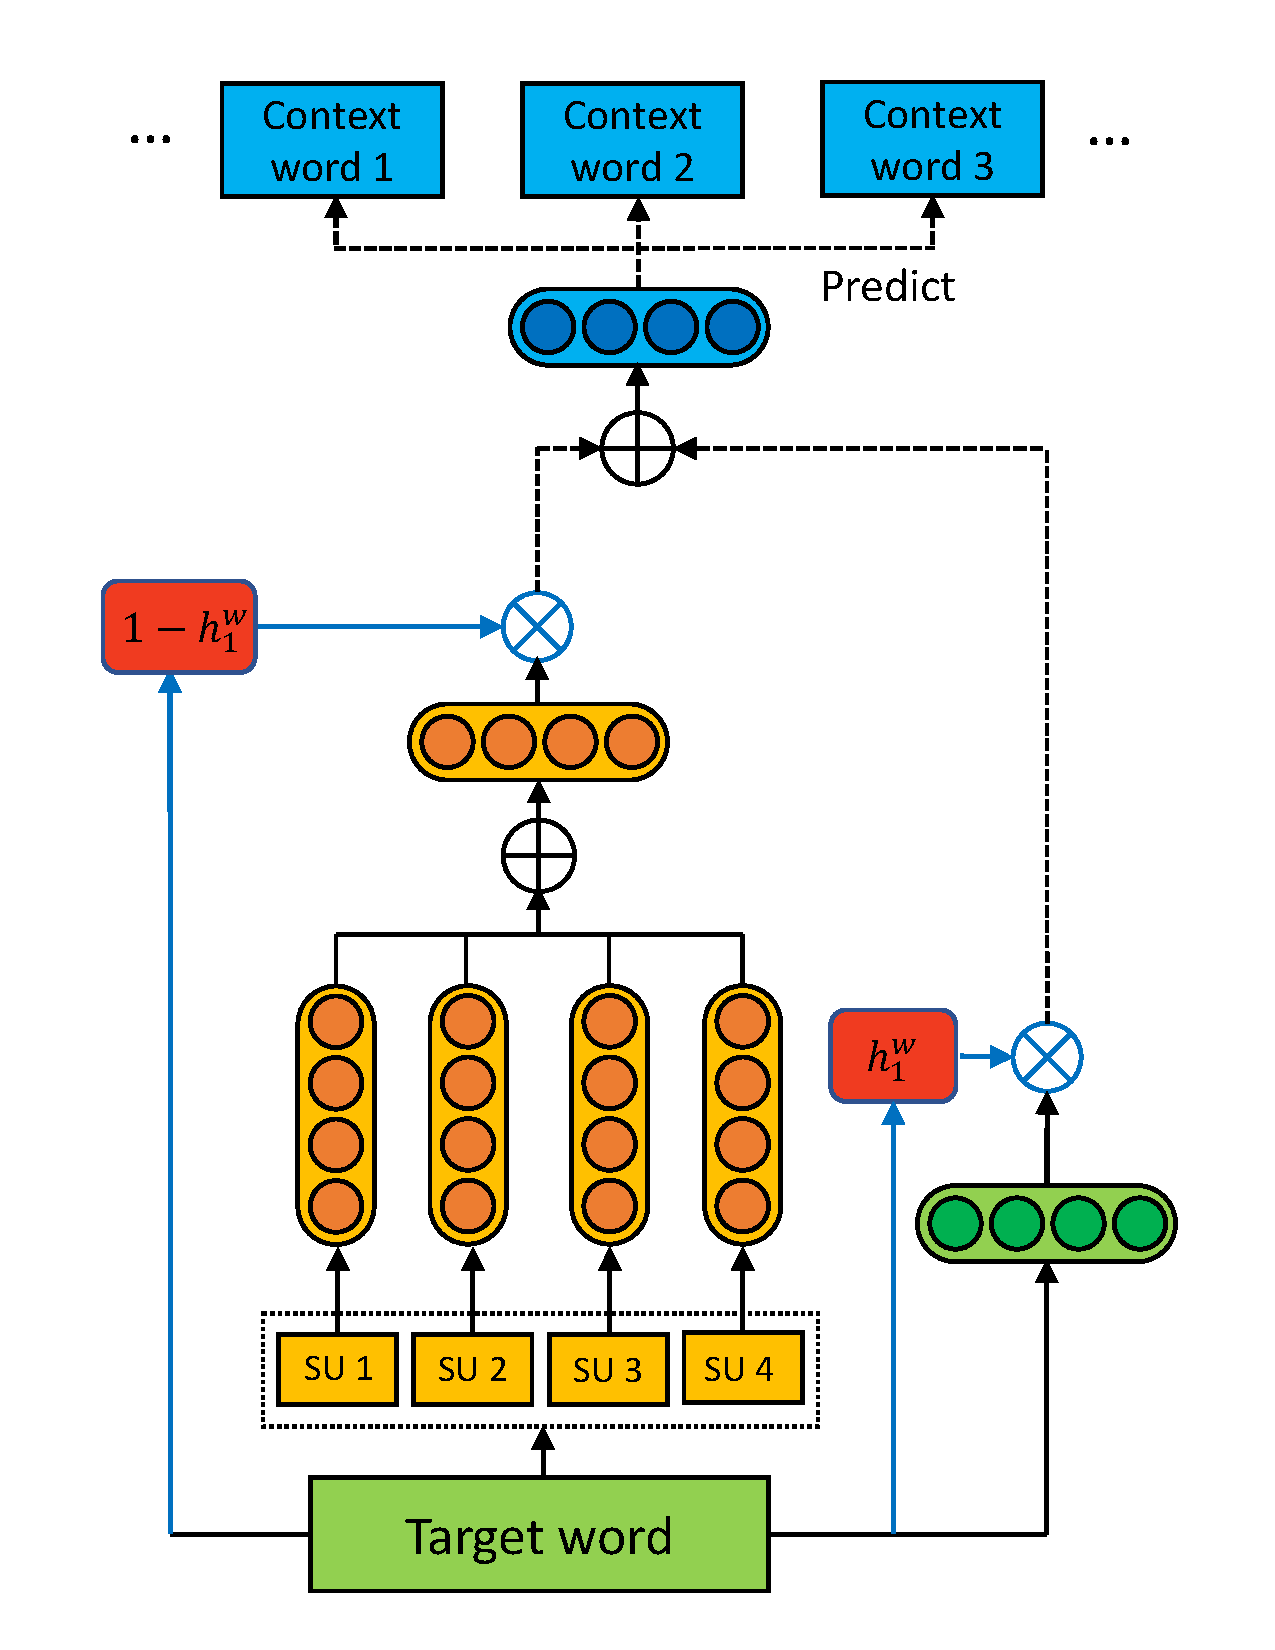
\includegraphics[width=\textwidth]{figures/XU_DSE-SG_subword.pdf}
	\caption{DSE-SG}
\end{subfigure}
\caption{The architecture of the two versions of the DSE model. DSE-CBOW associates a semantic weight parameter $h^w$ to each context word, and DSE-SG does this to each target word. The ``SU''s  in the yellow box stand for ``sub-word units''.}\label{fig:DSE}
\end{figure*}


In DSE, we use $h^w$ to compute the weighted average vector for each word, and substitute it for the average context vector $x_k$ in CWE (eq.~\ref{eq:CWE_avgvec}), and for the average target vector, as shown below:

\begin{equation}\label{eq:DSE_avgvec}
\begin{cases}
	x'_{k} = h^w_{k} v_k + (1 - h^w_k)\Big(\frac{1}{N_k}\sum^{N_k}_{t=1}{c_t}\Big), \\
		\quad\quad \text{replacing the } x_k \text{ in \cref{eq:CWE_avgvec}} \\
	x'_i = h^w_{i} v_i + (1 - h^w_i) \sum^{N_i}_{t=1}{c_t}, 
\end{cases}
\end{equation}
\noindent in which the subscripts $k$ and $i$ are the indices of words in the vocabulary. 
We have two versions of model architectures: one is based on CWE (CBOW-like), and the other is based on fastText (skipgram-like). They are referred to as \emph{DSE-CBOW} and \emph{DSE-SG} respectively.
The architectures of these models are shown in \Cref{fig:DSE}.

We call $h^w$ the semantic weight parameter. It describes the proportion of contribution from each word as an unanalyzable semantic unit, while $1-h^w$ is the total contribution from all the sub-word units.
$h^w$ is a learnable parameter in the model.


\subsection{Corpus data and training setup}
We use the Wikimedia database dumps\footnote{\url{https://dumps.wikimedia.org/}} (up until July 2017) as our training data. Data in six languages are used: Chinese (ZH), English (EN), French (FR), German (DE), Italian (IT) and Spanish (ES). Raw text data are extracted from the dump files using \texttt{WikiExtractor}.\footnote{ \url{https://github.com/attardi/wikiextractor}} Further text cleaning is conducted by separating sentences into lines, and converting non-proper-nouns (proper-nouns are identified using a pre-trained NER model provided in the Python package \texttt{spacy}\footnote{\url{https://spacy.io/}}) to lower case. 
For Chinese data particularly, word segmentation is carried out using the \texttt{Jieba} segmenter.\footnote{{\url{https://github.com/fxsjy/jieba}}} All traditional Chinese characters are converted to simplified characters using OpenCC\footnote{{\url{https://github.com/BYVoid/OpenCC}}}. All non-Chinese characters are removed, keeping only those within the Unicode range U+4E00--U+9FFF. 
The training data of all six languages are of similar volumes: 33 to 40 million tokens each after preprocessing. 

To accelerate training, we limit the number of effective semantic units in each word. For Chinese data, words containing more than 7 characters are ignored. For other languages, if a word contains more than 7 $n$-grams, we randomly select 7 out of them, and ignore the rest. Here the number 7 is chosen based on the following empirical observation: in a pilot study, we found that  numbers larger than 7 will not improve the resulting embeddings, but significantly slow down the training.  
Other hyper-parameters are kept as close to the previous studies as possible.  
The values of the hyper-parameters for training the DSE models are shown in \Cref{tab:hyperprams}.

\begin{table}
\begin{tabular}{l r}
\lsptoprule
Hyperparameter & Value \\
\midrule
Embedding size, word & 300 \\
Embedding size, sub-word & 300 \\
Window size & 5 \\ 
Number of negative samples & 10 \\
Batch size & 128\\
Minimal word frequency & 5 \\
Initial learning rate, DSE-CBOW & 0.05\\
Initial learning rate, DSE-SG & 0.025\\
\lspbottomrule
\end{tabular}
\caption{Hyperparameter setting for Study 1.}\label{tab:hyperprams}
\end{table}


The training stage consists of three steps: 

\begin{enumerate}
	\item Pre-train the word embeddings: set the parameters for word embeddings, i.e., the $v_k$ and $v_i$ in \Cref{eq:DSE_avgvec} to trainable; set all the other parameters to not trainable; train the model for 5 epochs.
	\item Pre-train the sub-word embeddings: set the parameters for sub-word units, i.e., $c_t$ in \Cref{eq:DSE_avgvec} to trainable; set all the other parameters to not trainable; train the model for 5 epochs.
	\item Set all the parameters to trainable (including embeddings and $h^w$s); train the model for 5 epochs. 
\end{enumerate}

As for the size of $n$-grams, we use a fixed size $n=4$, i.e., no bigrams or trigrams are considered. This choice is partially based on Bojanowski et al.'s \citeyearpar{bojanowski2017enriching} work showing that $n=4$ already achieves a satisfactory embeddings, and partially due to speed consideration. 
For words that consist of more than 4 letters, we only consider two sources for the mixture embeddings: the word itself and the $n$-gram ($n<4$).

The semantic weight parameters $h^w$ are implemented as a $V_w\times 1$ lookup table. Thus, in each training step, the learning algorithm updates three embedding tables: word embeddings $E_w$, character embeddings $E_c$, and the semantic weights. 
Specifically, for the DSE-SG model, the average embeddings are first computed from $E_w$, $E_c$, $h^w$, and $h^c$ using \cref{eq:DSE_avgvec} and then outputted as the final word vectors. For DSE-CBOW model, just the $E_w$ table is outputted as the learned word vectors.\footnote{The discrepancy exists in the original implementations of CWE and fastText, and the reason for it is out of the scope of this study.}


\subsection{Results and discussion}
We are interested in examining the relationship between the semantic weight $h^w$ of a word and its relative ``age''. 
According to the observation that Chinese is shifting from monosyllabic words to bisyllabic words, it is reasonable to expect that newer Chinese words should have larger $h^w$ than older words, because a higher $h^w$ indicates that the word as a whole rather than the individual sub-word units is more important in determining its meaning. 
For other languages, we do not have a clear idea on what the relationship could be, but they should provide an interesting comparison. 

\begin{figure*}[t]
\centering
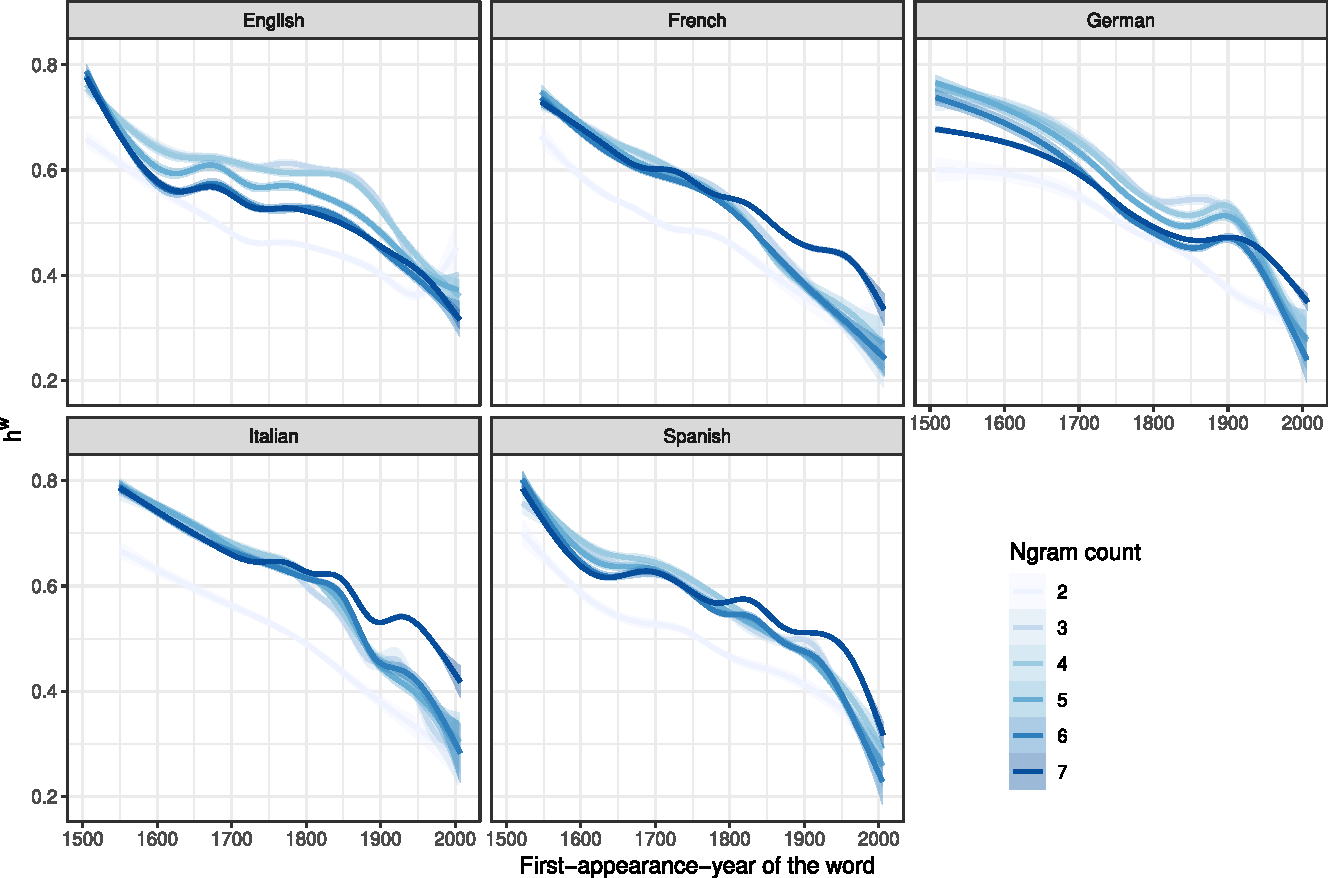
\includegraphics[width=\linewidth]{figures/XU_hw_year_ngramCount2to7_DSE_sg_wikiAllLangs}
\caption{Semantic weight $h^w$ against the first-appearance-year of words in DE, EN, ES, FR, and IT. Words with sub-word units ($n$-grams) number ranging from 2 to 7 are plotted separately. Shaded area indicates 95\% point-wise confidence intervals of the fitted regression lines. $h^w$ scores are from the DSE-SG model.}\label{fig:hw_year_fivelangs}
\end{figure*}

First, we need to have a reliable way to measure the ``age'' of a word. 
We use the Google Books Ngram (GBN)\footnote{ \url{http://storage.googleapis.com/books/ngrams/books/datasetsv2.html}} corpus, which contains word frequency information from about 10 million books published over a period of five centuries \citep{lin-etal-2012-syntactic}. 
It is the best resource we can find that provides estimated temporal distributions of words in multiple languages. 
For each word in GBN we extract the first \emph{year} it appears in the dataset, and use this first-appearance-year as an approximation of the word's age. Then we check if the word's age is correlated with its $h^w$ from training the DSE model. 
For example, the word {\cjkfont 爱人} \textit{ai ren} `lover' first appears in 1804 CE (at least according to the GBN collection).
Thus, our examination is based on the intersection of vocabularies between GBN and the training data. For DE, EN, ES, FR and IT, the intersection covers above $95\%$ of the most common words in the training set, and the proportion for ZH is $84\%$.\largerpage


In a short summary of the results, we find opposite $h^2 \sim \text{year}$ relationships in Chinese and the other five languages. 
$h^w$ decreases with the first-appearance-year in the five Indo-European languages, as shown in \Cref{fig:hw_year_fivelangs}. Words with sub-word units count ranging from 2 to 7 are included. Short words that have only 1 $n$-gram are excluded because the $n$-grams have the same form as the words. There are some fluctuations but the overall decreasing trends of $h^w$ are salient. 
As the decrease of $h^w$ is equivalent to the increase of $1-h^w$, it indicates that in these five languages, sub-word units carry more semantic weights in newer words than older ones. The $h^w$ scores reported in \Cref{fig:hw_year_fivelangs} are from the DSE-SG model.

As for Chinese, however, $h^w$ increases with the first-appearance-year as shown in \Cref{fig:hw_year_charNum234}. We choose the sub-word units (characters) count = $\{2,3,4\}$ because they are the majority in the training data, with proportions $57.5\%$, $31.0\%$, and $8.6\%$. Frequency-wise, their proportions are more dominant: $82.9\%$, $11.8\%$, and $4.6\%$ respectively. 
Single-character words are excluded because the vast majority ($98\%$) of words in the training data are multi-character ones.
Words composed of more than 4 characters are very uncommon in Chinese. 
From the plot, the increasing trends of the 2-character words are observable, but less so for the 3- and 4-character words.
This indicates that our hypothesis is supported: characters carry more semantic weight in older Chinese words than in newer Chinese words. 

Besides, an interesting finding is that the $h^w$s from DSE-SG are larger than those from DSE-CBOW in Chinese. It makes sense intuitively: a CBOW-like model is using multiple context words to predict one word, and thus the semantic weight of each individual word is diluted. 

\begin{figure}
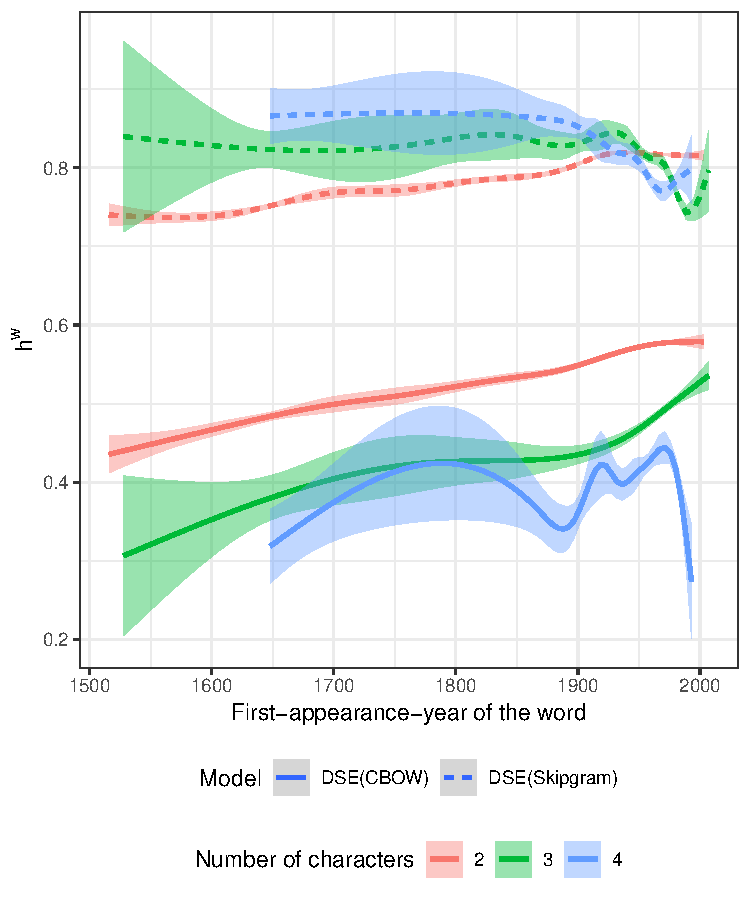
\includegraphics[width=0.55\linewidth]{figures/XU_hw_year_charNum234_cbow&sg_wikifull.pdf}
\caption{Semantic weight $h^w$ against first-appearance-year for Chinese words with character number = 2, 3, and 4. Shaded area indicates 95\% point-wise confidence intervals of the fitted regression lines.}\label{fig:hw_year_charNum234}
\end{figure}


\section{Study 2: Temporal patterns of semantic weight in historical corpora}\label{sec:study2}
In this study, we collect text data from Wikisource, a public resource of historical articles. We divide the text data into segments according to the years of authorship, and train embedding models on each segment individually. 
These individual models can reflect the semantic weight for each historical period, and we carry out a longitudinal analysis on how the semantic weight evolves. 

\subsection{Character-enhanced word embedding (CWE) model}
The model we utilize in this study is the character-incorporated word embedding models (CWE) \citep{chen2015joint}, which presents modifications on top of the original word2vec model. The design goal of CWE is to obtain a richer representation of Chinese words by assigning a vector to each character in a word. It replaces the context word vector, with an average vector $x_k$, 

\begin{equation}\label{eq:CWE_avgvec}
    x_k = \frac{1}{2}v_k + \frac{1}{2}\Big(\frac{1}{N_k}\sum^{N_k}_{t=1}{c_t}\Big)
\end{equation}
\noindent where $N_k$ is the number of characters in word $w_k$, and $c_t$ is the vector of the $t$th character. Here the weights on the word and the characters within that word are equal (0.5), which is based on an empirical hypothesis that context words and characters are equally important in determining the semantics of target word.


\subsection{Data collection and preprocessing}

Wikisource\footnote{\url{https://wikisource.org}} is part of the Wikimedia foundation,\footnote{\url{https://wikimediafoundation.org/}} which has the stated goal of developing and maintaining open content, wiki-based projects and providing the full contents of those projects to the public free of charge. 
It hosts text data from a broad range of categories and timespans, including professionally published articles, newspaper articles, archived documents, etc.
Wikisource includes multiple language-specific sub-domains with each article labeled with ``author'', ``title'', and ``publication time'' (with a yearly granularity). The largest sub-domains in terms of article number are English, French, Chinese, German, Spanish, and Russian. 
Thus, we include these six languages in this study.
The ProofreadPage extension makes sure that all the works on the website are verifiable, reliable, and accurate. 
Wikisource provides ancient (600 CE) as well as contemporary articles.
We therefore consider Wikisource a useful resource for building a corpus for historical language studies. Regrettably, only a few researchers have conducted research using this material. 

Wikisource does not offer direct download links of the data, so one of the challenges of this project is to acquire the textual data from the website. Furthermore, anyone can edit articles on the website, so the structure of each HTML page differs from the others. In order to solve this irregularity issue, distinctive web crawlers for each subdomain were developed and the crawled JSON data was extracted into text documents. 

The collected corpus contains articles from the 11th century to the 21st century; however, the number of articles is not evenly distributed along the timeline. The amount of textual data for each bin is very important for providing an accurate description of the semantics of a language for that time period. To overcome this difficulty, we will only consider the articles dated from 1820 to 1930. These articles were divided into temporal bins of 10 years. This division is arbitrary and it does not correlate with any semantic difference in the language. 
For this study, we use the Chinese subset of the corpus, because the target model CWE is designed for Chinese language only. 

\subsection{Word segmentation}
The Chinese written language is printed without marking boundaries between words, like the blank space that is commonly used in other languages. 
Thus, it requires a preprocessing step known as word segmentation, which places boundaries between adjacent characters in order to identify the unit of ``word''.
We use the \texttt{jieba} word segmentor\footnote{\url{https://github.com/fxsjy/jieba}} for this study. Although \texttt{jieba} is not designed for ancient Chinese, we found that it is able to detect words that belong to ancient vocabulary, such as {\cjkfont 中书} \textit{zhong shu} `an official position during the Tang dynasty', {\cjkfont 若夫} \textit{ruo ru} `if' etc.
The resulting corpus data with various word counts, character counts, and vocabulary sizes in terms of unique word tokens can be seen in \Cref{fig:corpus_stats}.

\begin{figure}
\centering
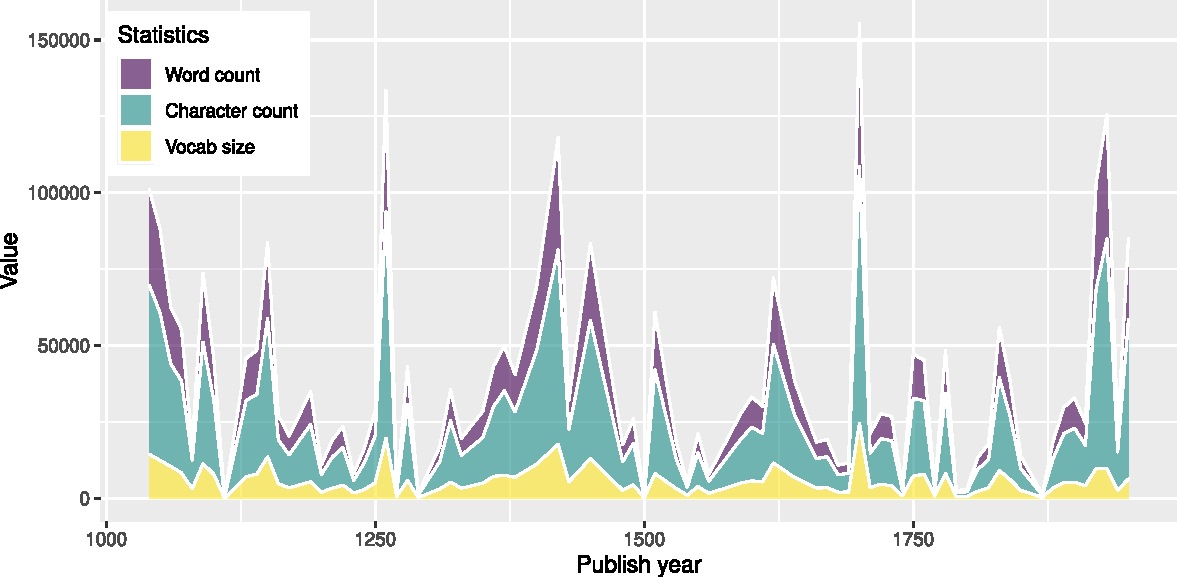
\includegraphics[width=\linewidth]{figures/XU_word_char_vocab_vs_year.pdf}
\caption{The distribution of word count, character count, and vocabulary size (number of unique words) across article publication years in the Wikisource corpora.}\label{fig:corpus_stats}
\end{figure}


\subsection{Definitions of semantic weight}
We define \emph{semantic weight} in a different way from that of Study 1 (Section~\ref{sec:study1}). Here, it is defined as the proportion of the Euclidean norm of a word vector relative to the mean norms of its constituent character vectors, designated by the $\Omega$ in \Cref{eq:semantic_weight_def2},

\begin{equation}\label{eq:semantic_weight_def2}
	\Omega_{w} = \frac{\lVert v_{w} \rVert}{\frac{1}{N_w}\sum_{c \in w}\lVert v_{c} \rVert + \lVert v_{w} \rVert}
\end{equation}
where $N_w$ is the number of characters in word $w$. $v_c$ is the embedding vector of character $c$, and $v_w$ is the word embedding vector. $\lVert v_w \rVert$ and $\lVert v_c \rVert$ are the Euclidean norms, which have theoretically unbounded positive values. 
A word with larger word vector norm $\lVert v_w \rVert$ will have a larger $\Omega_{w}$ score, while a word with a larger mean character norm $\lVert v_c \rVert$ will have a smaller $\Omega_{w}$ score.
Thus, $\Omega_w$ quantifies the degree to which a word functions as a whole semantic unit as opposed to its constituent sub-units. 
Since CWE has two versions of implementation, CBOW and Skipgram based, we examine both and use CWE-CBOW and CWE-Skipgram to refer to the models respectively.


\subsection{Model training procedure}
We first split the training data into segments, based on the publication year of the individual articles, and train one embedding model for each segment. 
We need to choose the size of segments carefully, because we need to have sufficient number of segments in order to find a consistent temporal pattern, while it is also necessary to make sure that each segment is sufficiently large so that the embedding models are effectively trained. It is basically a trade-off between granularity and effectiveness. 

The whole training set, designated by $\mathcal{D}$, is segmented into $N$ segments, resulting in $\{\mathcal{D}_1,\mathcal{D}_2,\dots,\mathcal{D}_N\}$. We experimented with $N=5$ and $N=10$. 
Since the token numbers are not evenly distributed among years, the size of $\mathcal{D}_i$ varies. In order to eliminate the potential confounding effects due to the varying sizes of training data, we randomly sample 30k lines of text from each $\mathcal{D}_i$ into $\mathcal{D}'_i$. 

For each $\mathcal{D}'_i$ in $\mathcal{D}$ ($i=1,\dots,N$; $N=9$), we train a CWE model, and calculate the $\Omega_w$ score for each word in vocabulary $V'_i$. Then we use the mean score $\smash{\Omega_i = \frac{1}{T_i}\sum_{w\in V_i}\Omega_w}$ to estimate the average semantic weight of historical period $i$. 
The purpose is to examine the relationship between $\Omega_i$ and $i$. Our assumption is that a correlation between $\Omega_i$ and $i$ should be observed. 


\subsection{Results and discussion}

We plot the $\Omega_i$ score against the historical period $i$ in \Cref{fig:omega_year}. It can be seen that $\Omega_i$ decreases as $i$ increases. Because larger values of $i$ represent the historical periods closer to modern time, the observed increasing trend indicates that words in modern languages have smaller $\Omega_i$ than words in ancient times. The same trends hold for both CWE-CBOW (\Cref{fig:omega_year_cbow}) and CWE-Skipgram (\Cref{fig:omega_year_skipgram}).

In order to make a less biased comparison, in \Cref{fig:omega_year} we individually observe words of different lengths, $l=1,2,3,4$. The $l=1$ group includes mono-character words, such as {\cjkfont 一} \textit{yi} `one', {\cjkfont 三} \textit{san} `three', {\cjkfont 万} \textit{wan} `ten thousand', etc. The $l=2$ group includes bi-character words, such as {\cjkfont 一定} \textit{yi ding} `must', {\cjkfont 不能} \textit{bu neng} `cannot', {\cjkfont 世事} \textit{shi shi} `world affairs' etc. The $l=3$ and $l=4$ groups contain more proper nouns (person and organization names), and fixed idioms, such as {\cjkfont 士大夫} \textit{shi da fu} `scholars', {\cjkfont 皇太后} \textit{huang tai hou} `queen', {\cjkfont 都督府} \textit{du du fu} `governor's office', etc. 
We fit individual linear models with formula $\Omega_i\sim i$ for all four length groups, and all models return statistically significant negative coefficients ($p<0.05$), indicating that the observed decreasing trends are reliable. The fitted regression lines and the bootstrapped 95\% confidence intervals are shown in \Cref{fig:omega_year}.

Another fact worthy of note is that only a small subset of words appears throughout the whole time span. For the accuracy of demonstration, we include only those words that exist in all nine vocabulary sets $V_i (i=1,2,\dots,9)$, which we refer to as \emph{common vocabulary}. The size of the common vocabulary is negatively correlated with word length, which is expected as an prediction of Zipf's law \citep{li1992random}. 

\begin{figure}
\centering
\begin{subfigure}{0.65\linewidth}
\centering
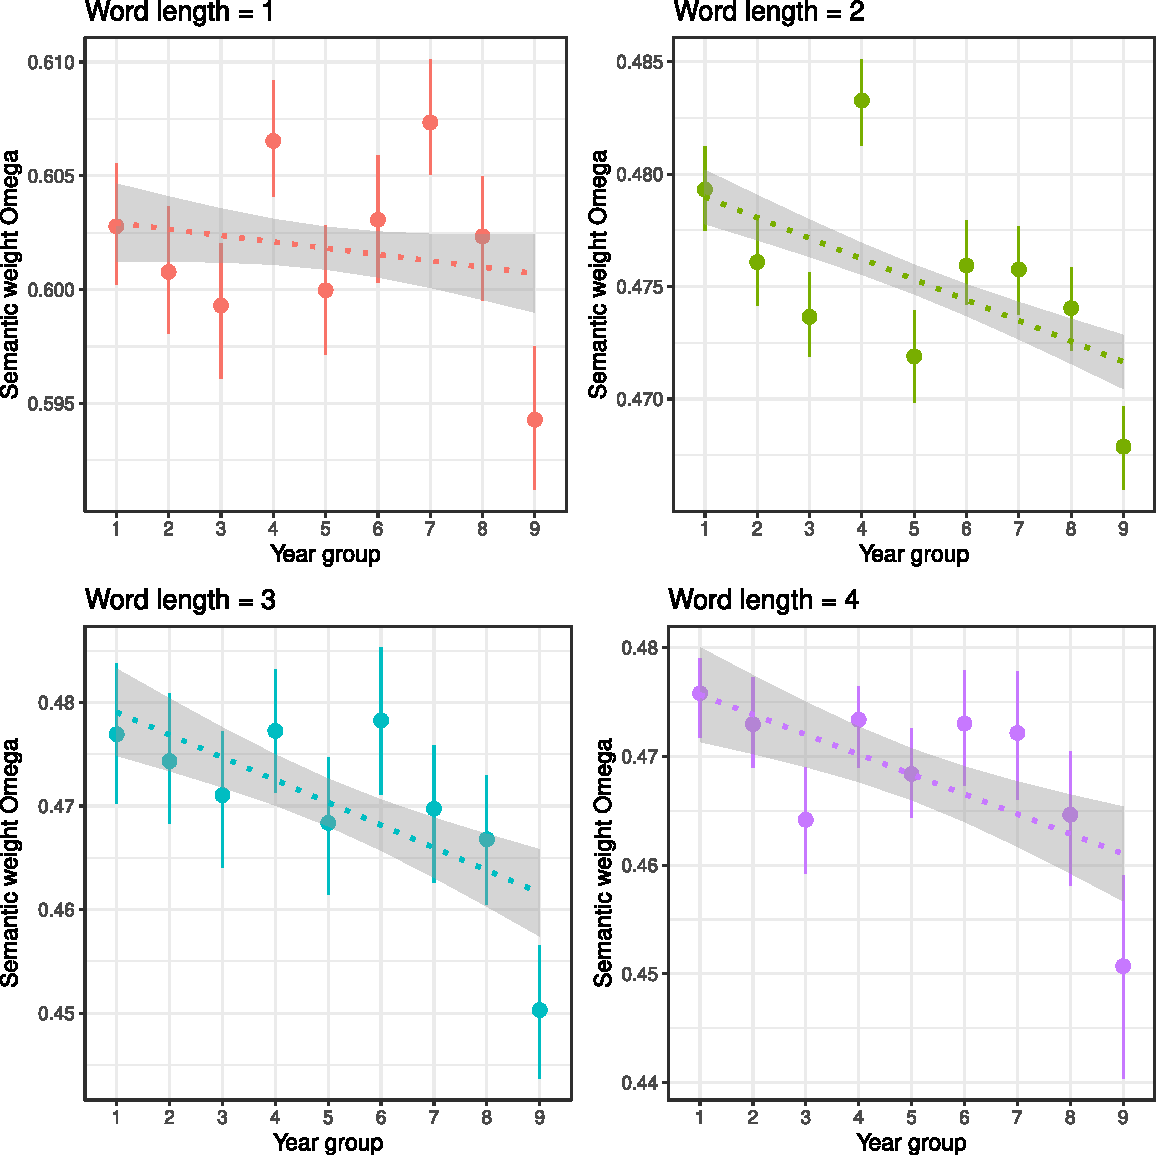
\includegraphics[width=\textwidth]{figures/XU_Omega_cbow_yeargroup_alllens_commonVocab_2by2}
\label{fig:omega_year_cbow}
\caption{Results from CWE-CBOW.}
\end{subfigure}\\
\begin{subfigure}{0.65\linewidth}
\centering
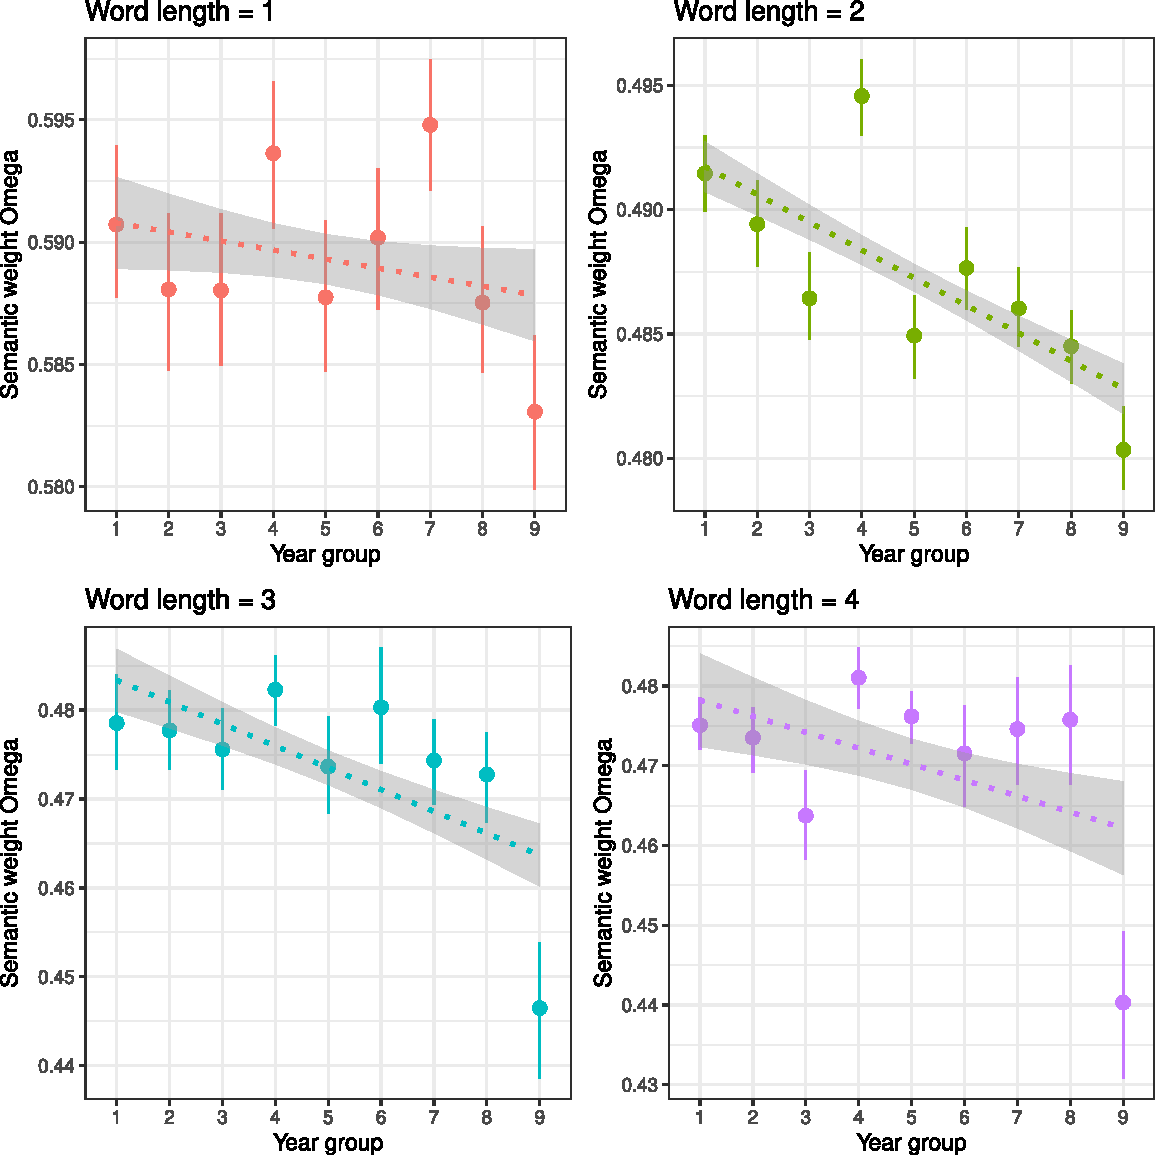
\includegraphics[width=\textwidth]{figures/XU_Omega_skipgram_yeargroup_alllens_commonVocab_2by2}
\label{fig:omega_year_skipgram}
\caption{Results from CWE-Skipgram.}
\end{subfigure}
\caption{Average semantic weight $\Omega_i$ in nine (9) historical groups ($i=1,2,\dots,9$). The results from CWE-CBOW and CWE-Skipgram are shown in (a) and (b) respectively.}\label{fig:omega_year}
\end{figure}


It is surprising to find that the $\Omega$ metric demonstrates contrary patterns as compared with the $h^w$ metric in Study 1. The semantic weight $\Omega$ demonstrates an opposite pattern compared with the $h^w$ coefficient defined in Study 1. 
In Study~1, the main finding about Chinese described in \Cref{fig:hw_year_charNum234} shows that the semantic weight measured by $h^w$ increases with the age of a word. The $\Omega$ in Study 2 shows a clear decreasing trend with historical period.

However, we do not think the results from Study 2 are sufficient to totally reject the conclusion from Study 1. First, the $x$ axis in Study 1 is the approximated ``age'' of a word, acquired from an external dictionary book (Google Books Ngram), while the $x$ axis in Study 2 is the \emph{actual} publication year. The independent variables of the two studies are essentially different. 
Based on the results, we lean towards Study 2 because the decreasing pattern of $\Omega$ in Chinese is consistent with those of the five Indo-European languages (\Cref{fig:hw_year_fivelangs}). We suspect that the age of Chinese words according to GBN may not be an accurate estimate. 
Secondly, the way we obtain $h^w$ and $\Omega_w$ is different as well. $h^w$ is automatically learned from data during the training stage of DSE model, while $\Omega_w$ is a post-hoc quantity computed after the CWE model is trained. In theories of representation learning \citep{bengio2013representation}, more informative parameters are assigned with larger weights by the model, thus $h^w$ and $\Omega_w$ should bear the same semantic weights. 
Based on these considerations, we conjecture that the discrepancy between Studies 1 and 2 is primarily due to the different operational definitions of historical periods. 
Beyond that, the empirical findings from both studies clearly indicate that the semantic weights of sub-word units indeed change with historical periods, confirmed by multiple corpora and models.  


\section{General discussion and conclusions}

The findings from Study 1 provide new evidence to linguistic theories about word formation. 
First, what constitutes a word in Chinese has changed: compared to its earlier stage, modern Chinese tends to have multiple characters for a single semantic unit. The semantic weight carried by a single character is decreasing. This is strong evidence in favor of the claim in qualitative studies that Chinese has been evolving towards multisyllabicity from monosyllabicity. 
Second, the trend of increasing semantic weights on sub-word units in Indo-European languages is consistent with the ``synthetic $\rightarrow$ analytic'' pattern shift at the phrase level composition \citep{hamilton-etal-2016-diachronic}. 
Moreover, the relative ``synthetic'' way of composing Chinese word found in this study seems consistent with the holistic encoding hypothesis in the perceptual theories about the Chinese writing system \citep{dehaene2005neural,mo2015holistic}. 

However, the above conclusions are not directly supported by the findings from Study 2. 
Both the $\Omega_w$ and $h^w$ quantify the role that a word itself as an atomic unit is playing in contributing to the semantic meanings, when sub-word units are also contributing to the meaning. $\Omega$ and $h^w$ should be of smaller value if sub-word units carry critical semantic information; they should be of greater value if sub-word units are not contributing actively. 
Thus, we believe the magnitudes of both quantities should correctly reflect the semantic importance played by sub-word units. 
Purely from the results of Study 2, we can also argue that the individual characters in Chinese are playing more and more important roles as the language evolves.
The inconsistency between Study 1 and 2 is primarily due to the different ways of setting up historical periods. In Study 1, we use the first year in which a word appears in a large collection of printed materials, which is less accurate than the segmentation method by actual publication year in Study~2. 

The usage of Google Books Ngram (GBN) dataset in Study 1 can be the direct cause for the inconsistency from Study 2. The lexicon publication year information in GBN is obtained from the OCR scans, which may suffer from missing pages or misrecognition. The main advantage of GBN is its support for multiple languages. For future work, more accurate resources for identifying word ages should be explored. For example, the Oxford English Dictionary \citep{oed} is a better resource for English, as it records the ambiguities and semantic changes for a large vocabulary of English, which can be used to identify the ``birth'' year of specific word meanings. 
Another planned improvement is to extend the range of sub-word units explored other than morphemes, for example, semantically-associated sub-word units such as phonesthemes \citep{bergen2004psychological,sagi2019taming}, sound symbolism \citep{imai2008sound} etc., because we assume the sub-word level semantic decomposition is ubiquitous, and should go beyond the predefined concepts of morphemes. 

Regardless of the seemingly conflicting results of the two studies presented in this chapter, we believe some meaningful empirical findings are discovered. First of all, the semantic weight of sub-word units can be quantified by well designed computational models. The parameters in those unsupervised machine learning models can provide interesting information that is not available with other count based statistical tools. 
Though we need to be careful when choosing proper models and proper ways of defining the computational metrics of semantic weights in future studies. At least fine-grained embedding models such as DSE and CWE should be further examined in terms of their behavioral consistency. 
More importantly, the semantic weights of sub-word units indeed demonstrate a clear pattern of change along historical periods, which to the best of our knowledge, is not discussed in previous studies. The semantic weights defined in this study can be viewed as a metric of the ``atomicness'' of words. We put forward a dynamic theory of word and sub-word level semantic composition -- the way we compose words, invent new words, and reuse old words, can be governed by some universal rules. What these rules are, and how they are related to the linguistic capacity of human beings are the research questions that await future work.


\section*{Acknowledgements}
We thank Nika Nizharadze for his effort in collecting and preprocessing the text data. We are grateful to Adam Jatowt for his great help in the preparation of this chapter. We appreciate the hard work from all the reviewers and editors. 

\section*{Abbreviations}
\begin{tabularx}{\textwidth}{@{}lQ@{}}
CBOW & continuous bag-of-words\\
CWE & character-enhanced word embedding\\
DSE & dynamic sub-word-incorporated embedding\\
GBN & Google Books Ngram\\
HTML & Hypertext Markup Language\\
JSON & JavaScript Object Notation\\
NER & named entity recognition\\
OCR & optical character recognition\\
SG & skipgram\\
\end{tabularx}


{\sloppy\printbibliography[heading=subbibliography,notkeyword=this]}
\end{document}
